\chapter{Motivation}
\label{motivation}

The goal of this thesis is to create a network that can be analyzed in the hope of understanding the causes of side effects for any drug represented in the network. The assumption is that a relationship triangle can be created in which chemicals, targets and phenotypes are associated with each other, see Figure ~\ref{fig:triangle}. In which case, the cause of side effects can be understood by analyzing the mechanism of action of drugs.

\begin{figure}[!ht]
    \centering
    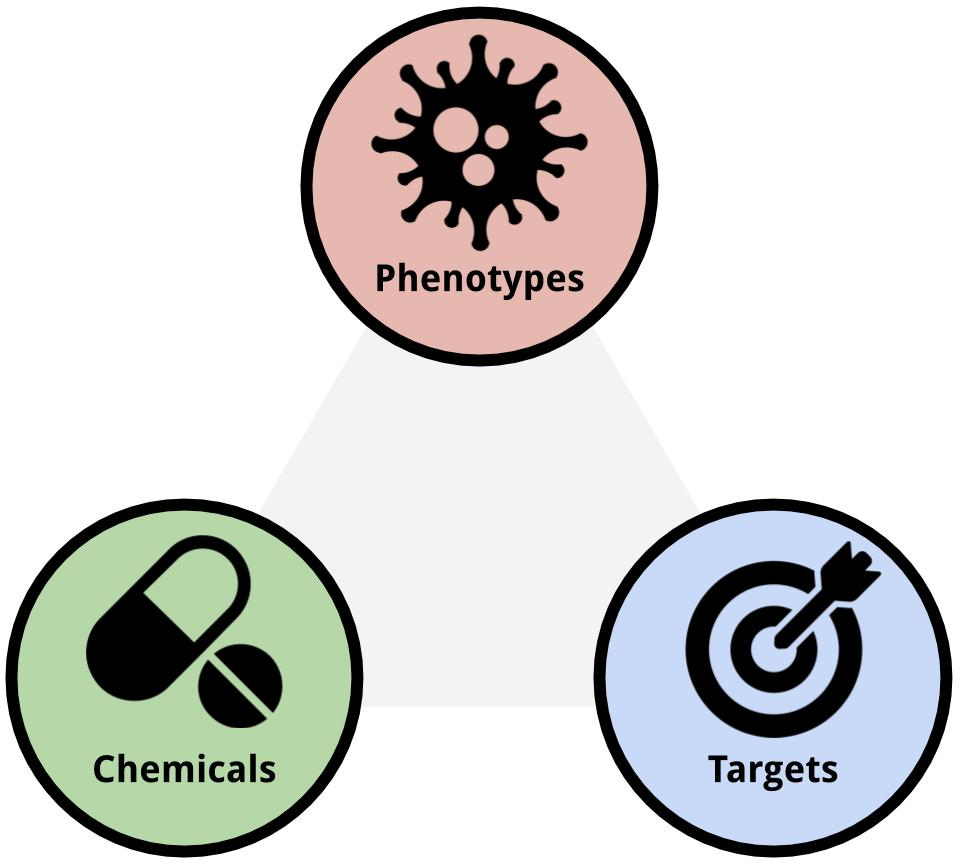
\includegraphics[scale=0.175]
    {figures/triangle.jpg}
    \caption{\label{fig:triangle} Chemicals-targets-phenotypes relationship triangle.}
\end{figure}

To achieve the goals of the project, first, a knowledge graph was created and enriched from multiple sources. This graph contained three different types of entities: chemicals, targets, and phenotypes; and three different relations, chemical-chemical, chemical-target and chemical-phenotype. Then, various \ac{NRL} approaches were used to create embeddings of the graph, which were then trained and optimized to obtain the best predictive model. This model was used to predict new relations with different node types, which were then analyzed using literature. A schematic of the workflow is presented in Figure ~\ref{fig:workflow}.

\begin{figure}[!ht]
    \centering
    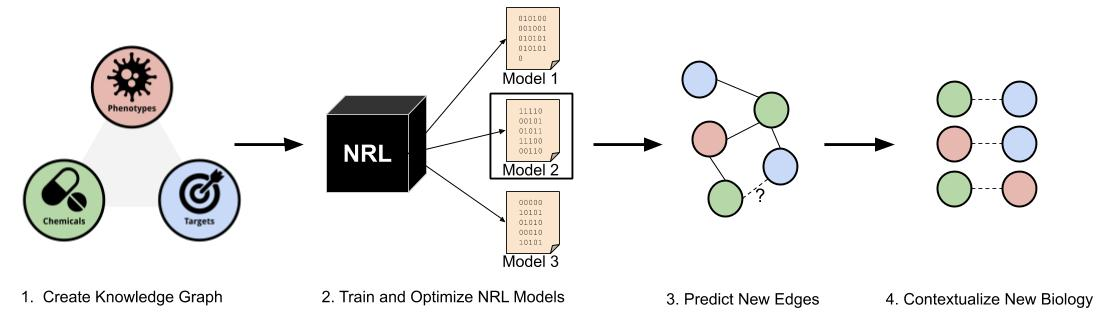
\includegraphics[scale=0.39]
    {figures/workflow.jpg}
    \caption [The workflow of the project]{\label{fig:workflow} The workflow of the project. 1. Create knowledge graph that contains chemicals, targets and phenotypes. 2. Train different NRL models and optimize them. 3. Use the best NRL model to predict new edges. 4. Contextualize the new knowledge.}
\end{figure}